\chapter{Anhang}

\section{Backpropagation und das Gradientenverfahren} \label{Backprop_GD}
Nachdem nun alle Agenten-Klassen vorgestellt sind, man sich vielleicht der eine oder andere Leser frage, wie denn nun das eigentliche Lernen vonstattengeht. Die dem Lernen zugrunde liegenden Verfahren sind das Backpropagation und das Gradient Descent. Dabei wird häufig fälschlicherweise angenommen, dass sich hinter dem Begriff Backpropagation der komplette Lernprozess verbirgt. Dem ist jedoch nicht so.\\
Der Backpropagation-Algorithmus oder auch häufig einfach nur Backprop genannt, ist der Algorithmus, welcher zuständig für die Bestimmung der Gradienten in einer Funktion. Häufig wird ebenfalls angenommen, dass Backprop nur für NN anwendbar sind, den ist jedoch nicht so. Prinzipiell können mit dem Backprob-Algorithmus die Gradienten einer jeden Funktion bestimmt werden, egal ob NN oder eine Aktivierungsfunktion, wie z.B. Sigmoid oder TanH \cite[S. 90ff.]{DL}.\\
\\Das Gradientenverfahren oder im Englischen auch Gradient Descent genannt, wird dafür eingesetzt um die eigentliche Optimierung des NN durchzuführen. Dafür werden jedoch die Gradienten benötigt, welche im Vorhinein durch den Backprop-Algorithmus bestimmt wurden. Jedes NN definiert je nach den Gewichten des NN eine mathematische Funktion. Diese steht in Abhängigkeit von den Inputs und berechnet auf deren Basis die Outputs bzw. Ergebnisse. Basierende auf dieser Funktion lässt sich eine zweite Funktion definieren, die Loss Function oder Kostenfunktion oder Verlustfunktion usw. Diese gibt den Fehler wieder und soll im Optimierungsverlauf minimiert werden, um optimale Ergebnisse zu erhalten. Diese Fehlerfunktion zu minimieren müssen die Gewichte des NN soweit angepasst werden, der die Fehlerfunktion geringe Werte ausgibt. ist diese für alle Daten, mit welchen das NN jemals konfrontiert wird geschafft, so ist das NN perfekt angepasst \cite[S. 225ff.]{DL}.\\
\\Ein näheres Eingehen auf die Bestimmung der Gradienten im Rahmen des Backpropagation-Algorithmus und auf die Anpassung der Gewicht im Rahmen des Gradientenverfahrens wird der Übersichtlichkeit entfallen. Des Weiteren machen moderne Framework wie Facebooks PyTorch, Googles Tensorflow oder Microsofts CNTK das detaillierte Wissen um diese Verfahren für anwendungsorientiert Benutzer obsolet.

\section{Tensoren}
Tensoren beschreiben die grundlegenden Einheiten eines jeden DL-Frameworks. Aus der Sicht der Informatik handelt es sich bei ihnen um mehrdimensionale Arrays, welche jedoch kaum etwas mit der mathematischen Tensorrechnung bzw. Tensoralgebra gemein haben. \cite[S. 67]{DRL_Lapan}
Genauer gesagt lassen sich Tensoren als, Anordnung von Zahlen in einem regelmäßigen Raster mit variabler Anzahl von Achsen. \cite[S. 35]{DL}\\
Ein DL-Framework kann aus z.B. einem Numpy Array \url{https://numpy.org/} einen Tensor konstruieren, welche dann über für die Verwendung in einem NN nutzbar ist. Dieser könnte Daten oder die gewichte eines NN beinhalten. Der entstandene Tensor dient dabei als eine Wrapper, welcher die Informationen des Arrays teilt oder kopiert hat. Neben vielen Zusatzfunktionen ist keine so wichtig wie das Aufbauen eines Backward Graphs. Ein DL-Framework ist mit diesem Graph in der Lage, jede Veränderung des Tensors einzusehen, um darauf aufbauend Backpropagation durchzuführen. \cite[S. 72 ff.]{DRL_Lapan}

\section{Convolution Neural Networks} \label{sec:Anhang_CNN}
Convolutional Neural Networks (CNNs) sind eine Form neuronaler Netzwerke, die besonders für das Verarbeiten von rasterähnlichen Daten geeignet sind. Sie bestehen meist aus verschiedenen Layers, wie z.B. Convolutional, Pooling und FC Layers.

\subsection{Convolutional Layer} \label{sec:Anhang_Conv_Layer}
Convolutional Layers (Conv Layers) sind der zentrale Baustein von CNNs, da sie besonders für die Feature Detektion geeignet sind. Ihre Gewichte sind in einem Tensor gespeichert. In diesen befinden sich die sogenannten Kernels oder auch Filter genannt, welche zweidimensionale Arrays darstellen. Bei Initialisierung der Conv Layers werden die Ein- und Ausgabe Channel der Inputs bzw. Outputs angegeben, sodass entsprechende dieser Informationen die Kernels erstellt werden können.\\
Des Weiteren wird noch die Größe der Kernels übergeben, wobei häufig Größen von (3x3), (5x5), (7x7) oder (1x1) genutzt werden.\\
\\Die Ausgabe eines Output Channels berechnet sich aus der Addition aller Input Channel Feature Maps, welche durch die Verrechnung mit den Kernels (Convolutionale Prozedur) entstanden sind. Für jeden Output Channel existiert ein Input Channel viele Kernel mit, daher ergibt sich eine Gewichtsmatrix der Form (Output\_Channel, Input\_Channel, Kernel\_Size[0], Kernel\_Size[1]) \cite[S. 369 ff.]{DL}\\
Die Funktionsweise der Convolutionalen Prozedur stellt sich wie folgt dar:\\
Jeder einzelne Kernel wird mit der Eingabe entsprechend \ref{fig:Conv2d} multipliziert und addiert. Ist dieser Berechnungsschritt abgeschlossen, bewegt sich das Eingabequadrat um dem sogenannten Stride weiter nach rechte (in der Grafik wird ein Stride von eins verwendet). Sollte ein Stride von zwei verwendet werden, so würde die Ausgabe $bw + cx + fy + gz$ nicht existieren und die resultierende Feature Map wäre kleiner. Daher wird der Stride gerne dazu verwendet, um die Feature Map Size und damit den Berechnungsaufwand zu senken. Des Weiteren lässt sich der Stride nicht nur in der Horizontalen sondern auch in der Vertikalen anwenden.\\
Nicht in \ref{fig:Conv2d} abgebildet ist das sogenannte Padding. Bei diesem wird an den Feature Maps weitere Nullzeilen bzw. Nullspalten angefügt. Dabei kann an allen vier Seiten oder an speziell ausgewählten Zeilen bzw. Spalten hinzuaddiert werden. Wie in \ref{fig:Conv2d} zu erkennen ist, hat die Feature Map die Form (3x4), jedoch ist der Output nur noch von der Form (2x3). Die Durchführung der Convolution Prozedur sorgt für eine Verkleinerung, welche durch Padding verhindert werden kann. \cite[S. 369 ff.]{DL}
Die Ausgaben in \ref{fig:Conv2d} bilden eine Feature Map, welche mit allen weiteren Feature Maps zusammenaddiert werden müsste um einen Output Channel zu bilden.
\begin{figure}[H]
	\centering
	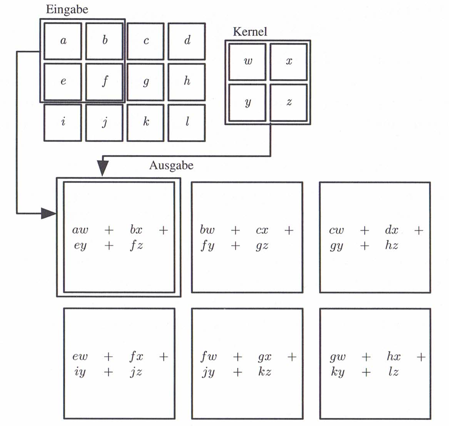
\includegraphics[scale=0.69]{Abbildungen/Anhang/Conv.png}
	\caption[Darstellung Convolutional Computation]{Darstellung der Berechnung einer 2-D-Faltung bzw. einer convolutionalen Prozedur. \cite[S. 373]{DL}}
	\label{fig:Conv2d}
\end{figure}

\subsection{Pooling Layer} \label{Pooling_Layer}
Pooling beschreibt die Minimierung der Feature Maps, wie es bereits in \ref{Conv_Layers} angesprochen wurde. Zu diesem Zweck wird in \ref{fig:Maxpool} ein Kernel und Stride der Form (2x2) gewählt, welcher ein Max-Pooling durchführen soll. Dieser Kernel bewegt sich über die Feature Map entsprechende des Strides und gibt den maximalen Wert innerhalb der Kernels wieder. Somit wird aus einer (4x4) eine (2x2) Feature Map. \cite[S. 379 ff.]{DL}

\begin{figure}[H]
	\centering
	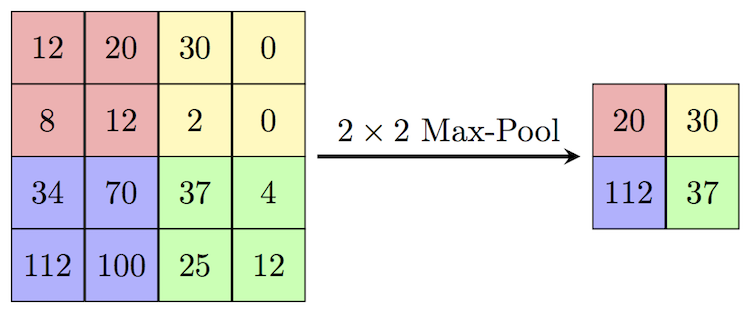
\includegraphics[scale=1.7]{Abbildungen/Anhang/Maxpool.png}
	\caption[Darstellung MaxPooling]{Darstellung des Max-Poolings. \url{https://computersciencewiki.org/images/8/8a/MaxpoolSample2.png}}
	\label{fig:Maxpool}
\end{figure}

\subsection{Fully Connected Layer} \label{FC_Layers}
Die Fully Connected Layer (FC) sind die grundlegendsten Elemente eines NN. Ein solches Layer besteht aus zwei Teilen, die beide einer Initialisierung benötigen.
Die Gewichte des FC sind als Tensor mit der Form (Anzahl der Output Features, Anzahl der Input Features) initialisiert. Zuzüglich kann optional noch ein Bias erstellt werden, welcher auf jedes Output Feature noch einen Rauschwert aufaddiert. Die Größe dieser Rauschwerte werden durch Backpropagation und Gradientenverfahren bestimmt, wie es auch bei den Gewichten der Fall ist. Die FC Layer implementieren daher folgende Funktion:
\begin{align}
	y = xA^T + b
\end{align}
wobei $y$ das Ergebnis, $x$ der Input Tensor, $A^T$ die Gewichte und $b$ das Bias, darstellt. \url{https://pytorch.org/docs/stable/generated/torch.nn.Linear.html}



